%\paragraph{Expected significance}
%
%The expected sensitivity of the Mono-Z(ll) channel to 2HDM+a models is approximated using generator level signal samples and background estimates from recent $Z(\ell \ell) + \MET$ searches using 36.1 \ifb of 13 TeV data \cite{Aaboud:2017bja}.  For signal events a reconstruction efficiency of 75\% is assumed, and to be consistent with the background estimates, the same selection cuts as \cite{Aaboud:2017bja} are used.  Signal and background are binned in \MET and a conservative background systematic of 20\% is assumed for $\MET < 120$ \GeV and 10\% above.
%
%Total significance is defined as the per bin significances summed in quadrature.
%
%\begin{equation}
%\mathcal{S} = \sqrt{\sum_{bin} (Z^\prime_{bin})^2}
%\end{equation}
%
%Following the Asimov approximation, the significance for individual bins is calculated as a Poisson ratio of likelihoods modified to incorporate  systematic uncertainties on the background  \cite{Cowan:2012}:  
%%(\autoref{eq:significance_wsyst})
%
%\begin{equation}
%\label{eq:significance_wsyst}
%Z^\prime_{bin} = \sqrt{ 2 \cdot \bigg( (s+b) \ln[\frac{ (s+b) (b+\sigma_b^2) } {b^2 + (s+b) \sigma_b^2} ]- \frac{b^2}{\sigma_b^2} \ln[1 + \frac{\sigma_b^2 s}{b(b+\sigma_b^2)} ] \bigg) }
%\end{equation}
%
%This metric has the advantage that it accounts for background systematics and is still valid for $s$ not $\ll b$.  Expected significances are shown in  \autoref{fig:expected_significance_monozll}, with regions the ATLAS and CMS experiments should be sensitive to, greater than 2, highlighted.
%
%%\begin{equation}
%%\label{eq:significance}
%%Z = \sqrt{2 \bigg( (s+b) \ln{1 + \frac{s}{b}} - S \bigg) }
%%\end{equation}
%
%
%\paragraph{Conclusions} The Mono-Z(ll) provides experimental coverage of the pseudoscalar 2HDM model for a broad part of the parameter space. The light pseudoscalar $a$ can be probed up to mass values of $\approx\unit[350]{GeV}$, depending on the choice of parameters. The Mono-Z channel is sensitive mostly in the region of $\tanb<4$.
%
%
%
%
%
%
%
%
%
%
%\begin{figure}
%\centering
%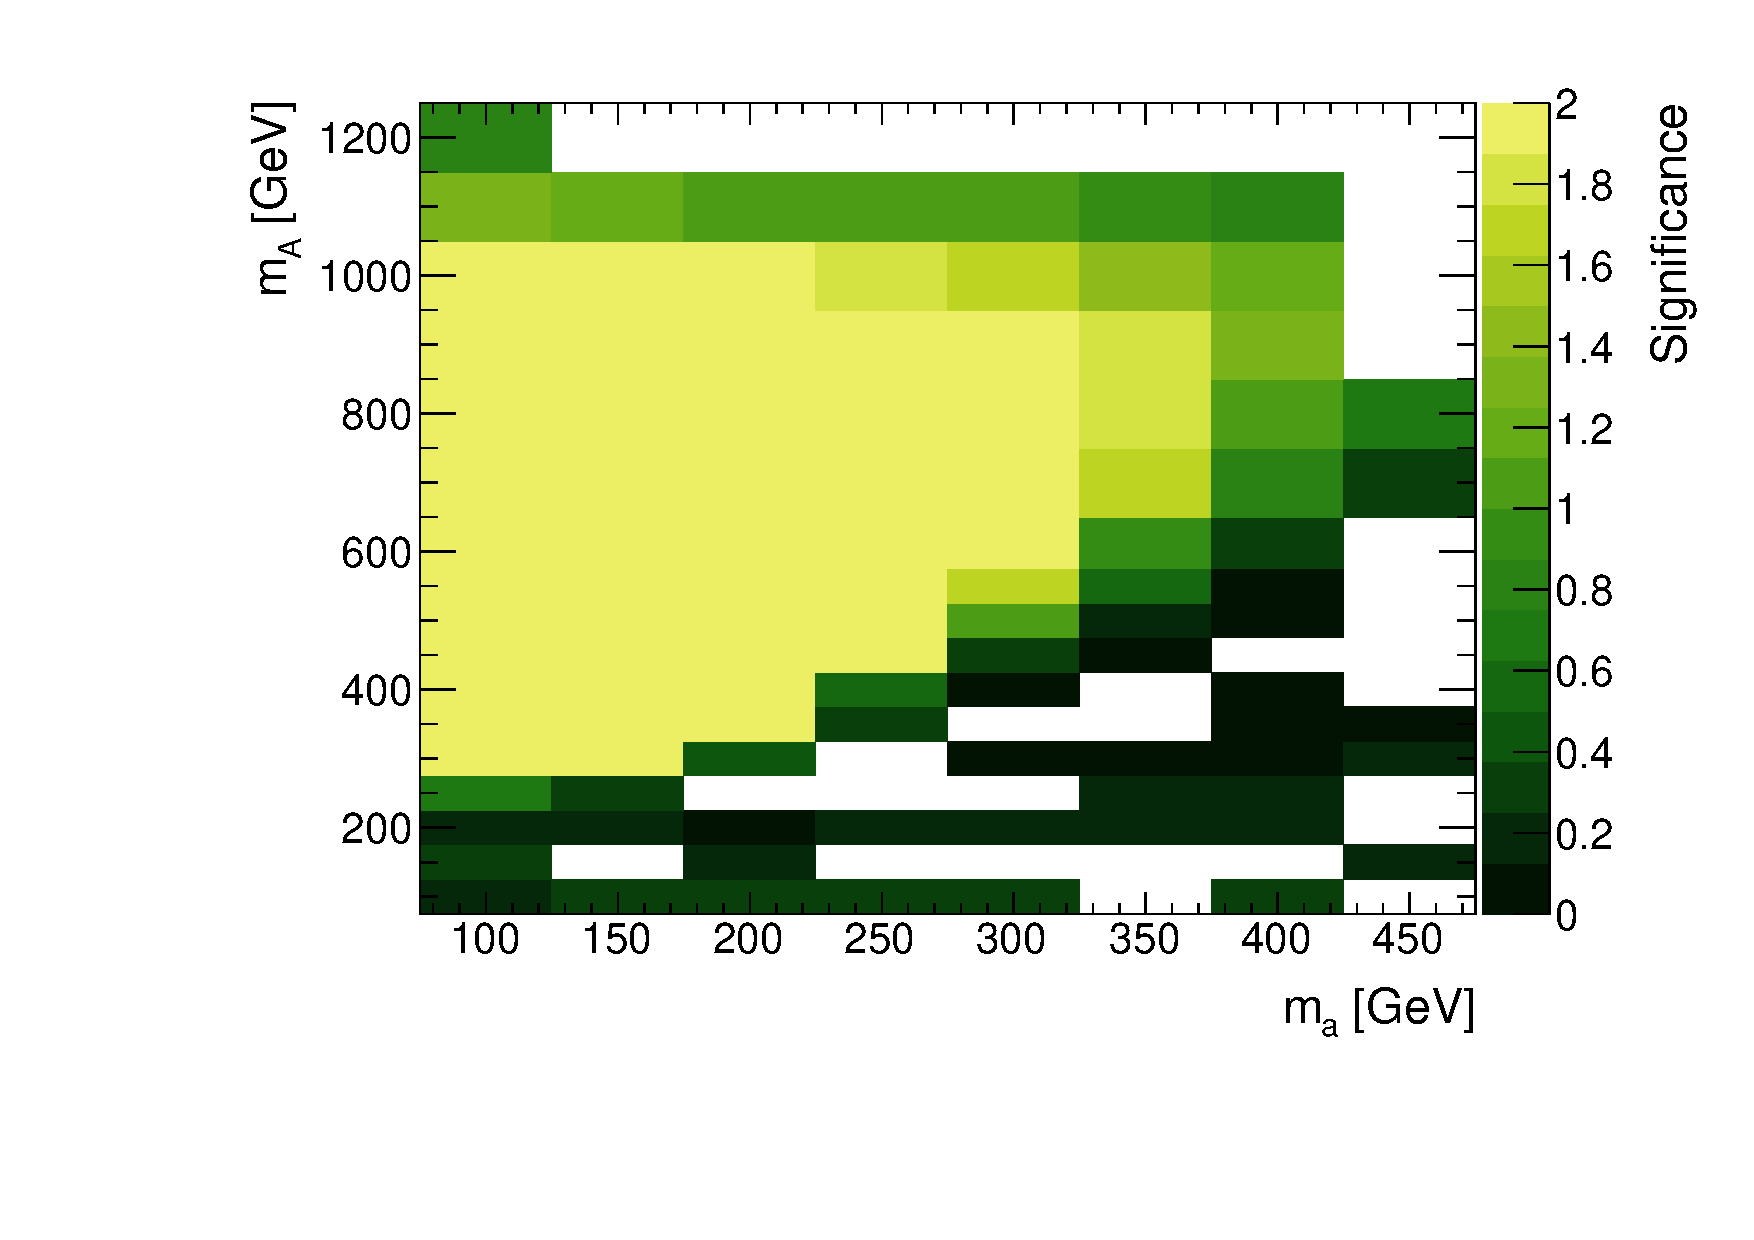
\includegraphics[width=0.6\textwidth]{texinputs/04_grid/figures/monoz/leptonic/mAma_Significance_ll.pdf}
%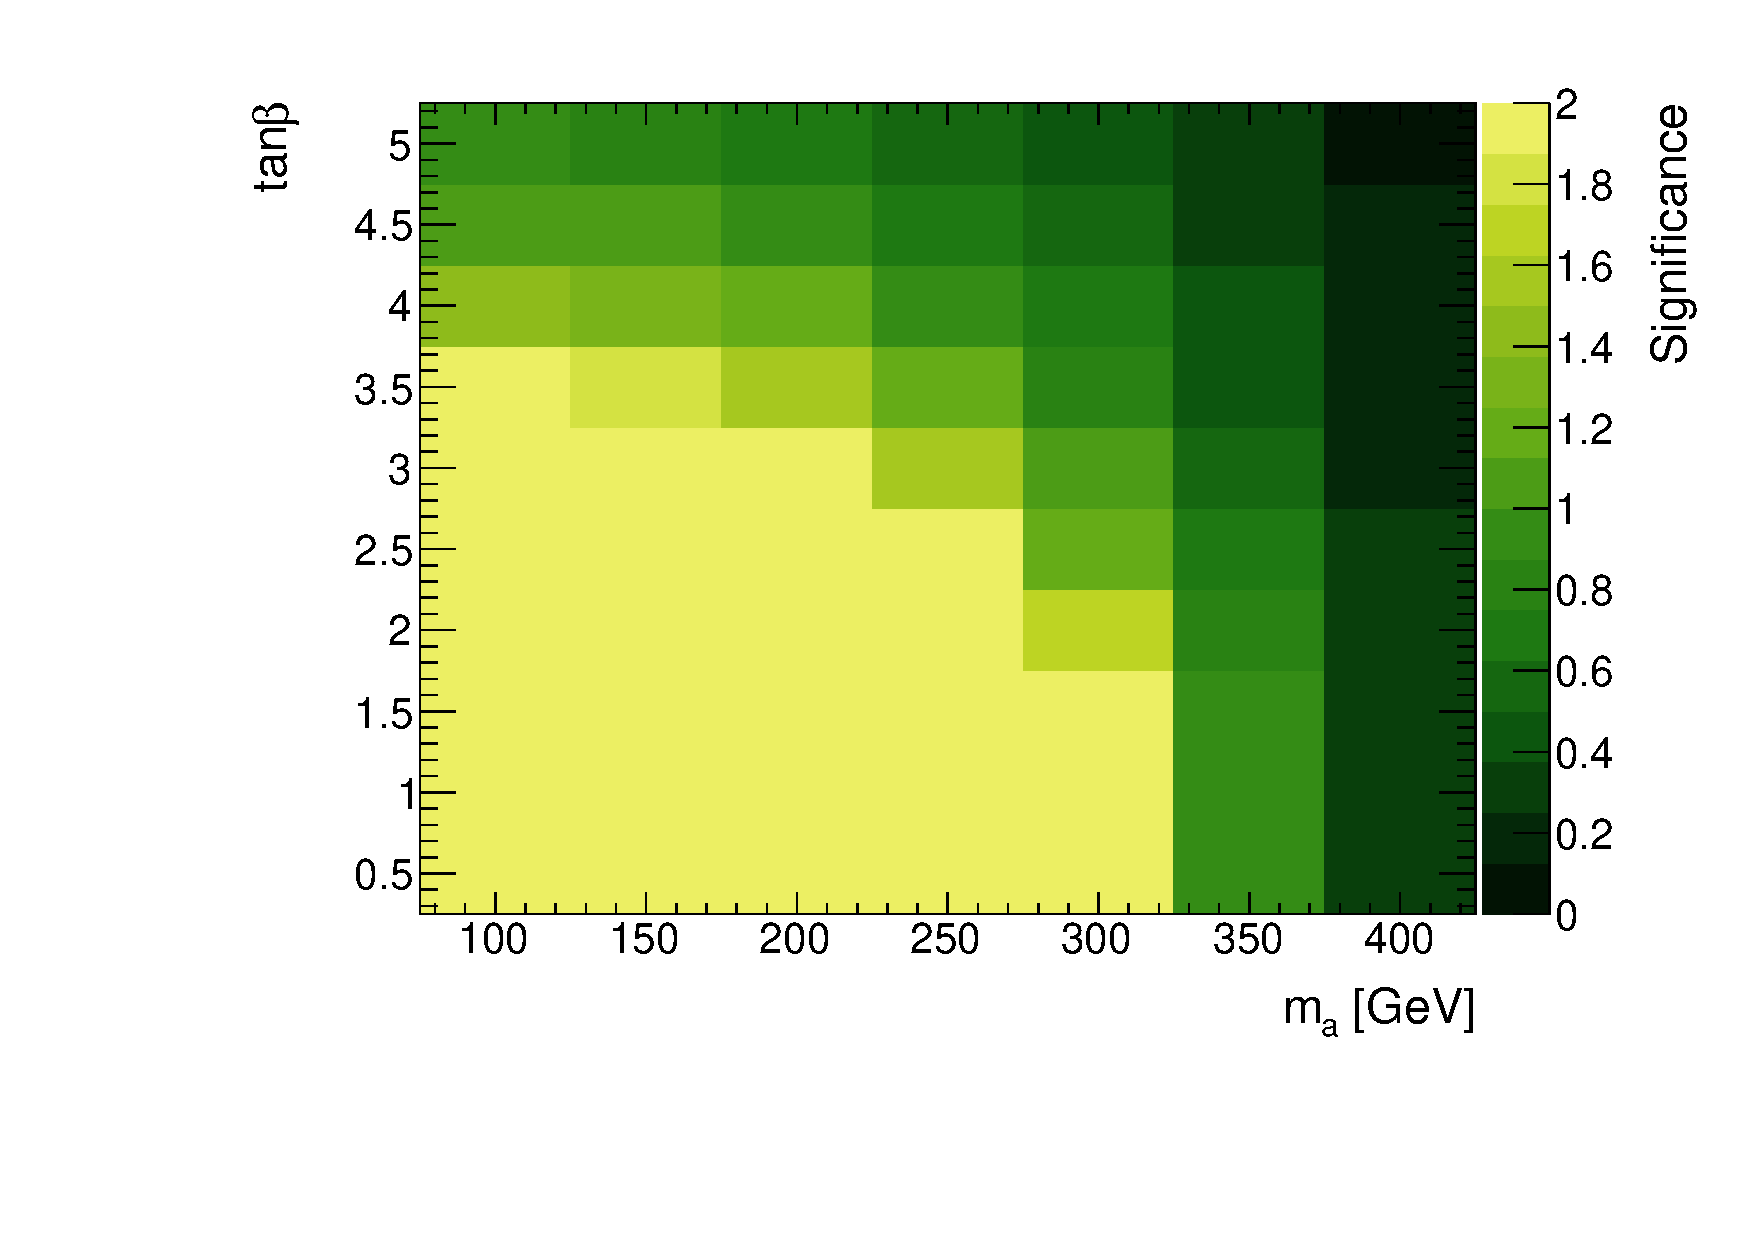
\includegraphics[width=0.6\textwidth]{texinputs/04_grid/figures/monoz/leptonic/tanbma_Significance_ll.pdf}
%\caption{Expected significances are calculated using published background estimates and assuming a reconstruction efficiency of 75\%.  The ATLAS and CMS experiments are expected to be sensitive to regions with significances greater than 2.}
%\label{fig:expected_significance_monozll}
%\end{figure}

